%% 
%% This is a sample doctoral dissertation.  It shows the appropriate
%% structure for your dissertation.  It should handle most of the
%% strange requirements imposed by the Grad school; like the different
%% handling of titles of one/many appendices.  It will automatically
%% handle the linespacing changes.  The body default is double-spaced
%% (except when you use the singlespace or condensed options).  The
%% default for quotations is single-space, and the default for tabular
%% environments is also single-space.  
%%
%% This class adds the following commands and environments to the
%% report class, upon which it is based:
%% Commands
%% ------------
%% \degree{name}{abbrv} -- Sets the name and abbreviation for the degree.
%%                         These default to ``Doctor of Philosopy''
%%                         and ``Ph.D.'', respectively.
%% \copyrightyear{year} -- for the copyright page.
%% \bachelors{degree}{institution} -- for the abstract
%% \masters{degree}{institution}   --  "
%%     if you have other degrees you may use
%% \secondbachelors{degree}{institution}
%% \thirdbachelors{degree}{institution}
%% \secondmasters{degree}{institution}
%% \thirdmasters{degree}{institution}
%% \priordoctorate{degree}{institution}
%%
%% \committeechair{name}           -- for the signature page
%% or, if you have two co-chairs:
%% \cochairs{first name}{second name}
%%
%% \firstreader{name}              --  "
%% \secondreader{name}             --  "
%% \thirdreader{name}              -- (optional)
%% \fourthreader{name}             --  "
%% \fifthreader{name}              --  "
%% \sixthreader{name}              --  "
%% \departmentchair{name}          -- for the signature page
%% \departmentname{name}           --  "
%%
%% \copyrightpage                  -- produces the copyright page
%% \signaturepage                  -- produces the signature page
%%
%% \frontmatter                    -- these are required in their various
%% \mainmatter                     -- appropriate locations
%% \backmatter                     --
%%
%% \unnumberedchapter[toc]{name}   -- like \chapter, except that it
%%                                    produces an unnumbered chapter;
%%                                    alternatively, like \chapter*,
%%                                    except that it lists the chapter
%%                                    in the table of contents.
%%
%% New environments:
%%   dedication  -- for the dedication
%%   abstract    -- for the abstract
%%
%% The thesis documentclass is built on top of the report document class.
%% It accepts all of the options that the report class accepts, plus the
%% following:
%%     doublespace -- the default, indicates double spacing as per U.Mass.
%%                    requirements.  You will need this when you do your
%%                    final copy.
%%     singlespace -- for earlier work, not acceptable to the Grad school
%%     condensed   -- for earlier work, not acceptable to the Grad school,
%%                    creates condensed versions of the frontmatter. 
%%                    Condensed implies singlespace.
%%     dissertation - the default, indicates that this document is a
%%                    dissertation.
%%     proposal    -- indicates that this document is a dissertation proposal,
%%                    rather than a dissertation.  This will only change the
%%                    wording on the title and signature pages.
%%     thesis      -- indicates that this document is a Master's thesis 
%%                    rather than a doctoral dissertation.  This also changes
%%                    the default for \degree to Master of Science, M.S.
%%     allowlisthypenation -- (the default), allows hyphenation of words in
%%                    the table of contents, the list of figures, and the list
%%                    of tables.  I believe that this is acceptable to the 
%%                    Graduate School.
%%     nolisthyphenation -- disallows hyphenation of words in the table of
%%                    contents and the list of figures and tables.  Use this 
%%                    option if the Grad School doesn't like your hyphenation.
%%     nicerdraft  -- relaxes some of the Grad School's rules for working with
%%                    drafts -- has no effect when doublespace is in effect
%%     nonicerdraft -- the default, leaves things in draft as they will be in
%%                     the final version
%% umassthesis changes the default font size to 12pt, but you may specify 10pt or
%%   11pt in the options.
\documentclass[12pt,honorthesis]{thesis}          % for Ph.D. dissertation or proposal
\usepackage{amsmath}
\usepackage{graphicx}
% \documentclass[thesis]{umassthesis}  % for Master's thesis

%%
%% If you have enough figures or tables that you run out of space for their
%% numbers in the List of Tables or List of figures, you can use the following
%% command to adjust the space left for numbers.  The default is shown:
%%
%% \setlength{\tablenumberwidth}{2.3em}

%% Use the hyperref package if you're producing a version for online
%% distribution and you want hyperlinks.  Note that the Grad School doesn't want
%% their PDF viewers to colorize or otherwise highlight the links; use the
%% hidelinks option to hyperref to avoid decorating links.
%\usepackage[hidelinks]{hyperref}

%% One way of formatting the epigraph/frontispiece is to use this package.
%\usepackage{epigraph}

\begin{document}

%%
%% You must fill in all of these appropriately
\title{Calibration for natural language processing systems}
\author{Khanh X. Nguyen}
\date{April 015} % The date you'll actually graduate -- must be
                     % February, May, or September
\copyrightyear{2015}
\bachelors{B.Sc.}{University of Massachusetts-Amherst}
% \committeechair{B. B. Bahh}
\cochairs{Brendan O'Connor}{Erik Learned-Miller}
%\fifthreader{}            % Optional
%\sixthreader{}            % Optional
\departmentchair{Benjamin Marlin} % Uses "Department Chair" as the title. To
% use an alternate title, such as "Chair", use \departmentchair[Chair]{Pete Shearer}
\departmentname{School of Computer Science}

%% If your degree is something other than a Ph.D. (for a dissertation), or
%% an M.S. (for a thesis), you will need to uncomment the appropriate
%% following line:
%%
%% \degree{Doctor of Education}{Ed.D.}
%% \degree{Doctor of Philosophy}{Ph.D.}
%%
%% \degree{Master of Arts}{M.A.}
%% \degree{Master of Arts in Teaching}{M.A.T.}
%% \degree{Master of Business Administration}{M.B.A.}
%% \degree{Master of Education}{M.Ed.}
%% \degree{Master of Fine Arts}{M.F.A.}
%% \degree{Master of Landscape Architecture}{M.L.A.}
%% \degree{Master of Music}{M.M.}
%% \degree{Master of Public Administration}{M.P.A.}
\degree{Bachelor of cience}{B.sc.}
%% \degree{Master of Regional Planning}{M.R.P.}
%% \degree{Master of Science}{M.S.}
%% \degree{Master of Science in Accounting}{M.S. Acctg.}
%% \degree{Master of Science in Chemical Engineering}{M.S. Ch.E.}
%% \degree{Master of Science in Civil Engineering}{M.S.C.E.}
%% \degree{Master of Science in Electrical and Computer Engineering}{M.S.E.C.E.}
%% \degree{Master of Science in Engineering Management}{M.S. Eng. Mgt.}
%% \degree{Master of Science in Environmental Engineering}{M.S. Env. E.}
%% \degree{Master of Science in Industrial Engineering and Operations Research}{M.S.I.E.O.R.}
%% \degree{Master of Science in Manufacturing Engineering}{M.S. Mfg. Eng.}
%% \degree{Master of Science in Mechanical Engineering}{M.S.M.E.}
%%
%% \degree{Professional Master of Business Administration}{P.M.B.A.}

%%
%% These lines produce the title, copyright, and signature pages.
%% They are Mandatory; except that you could leave out the copyright page
%% if you were preparing an M.S. thesis instead of a PhD dissertation.
\signaturepage

%%
%% Dedication is optional -- but this is how you create it
%%\begin{dedication}              % Dedication page
%%  \begin{center}
%%    \emph{To thos little lost sheep.}
%%  \end{center}
%%\end{dedication}

%%
%% Epigraph (aka frontispiece) is also optional, but this is one way you
%% can create it
%\begin{frontispiece}
%  %% Format to your liking -- see documentation of epigraph package
%  \setlength{\epigraphrule}{0pt}
%
%  \begin{epigraphs}
%    \qitem{%
%      \itshape
%      Mary had a little lamb,\\
%      Her fleece was white as snow.\\
%      \vspace{\baselineskip}
%      And everywhere that Mary went\\
%      The lamb was sure to go.
%      \vspace{\baselineskip}}
%    {Sarah Josepha Hale}
%
%    \vspace{2\baselineskip}
%    \qitem{%
%      \itshape
%      Baa, baa, black sheep,\\
%      Have you any wool?\\
%      Yes, sir, yes, sir,\\
%      Three bags full;\\
%      One for the master,\\
%      And one for the dame,\\
%      And one for the little boy\\
%      Who lives down the lane.
%      \vspace{\baselineskip}}
%    {English Nursery Rhyme}
%
%  \end{epigraphs}
%\end{frontispiece}

%%
%% Acknowledgements are optional...yeah, right.
%%
%% Abstract is MANDATORY. -- Except for MS theses

\begin{abstract}
  We argue that measuring the reliability of probabilistic predictions is crucial for mitigating cascaded errors and estimating risks in natural language processing systems. Hence, we propose \textit{calibration analysis} as a new tool for assessing the probabilistic predictions. Two methods are offered to present analysis results: calibration score and calibration curve. We show that they can be effectively estimated using a simple non-parametric regression method. Moreover, confidence intervals of the estimates can also be constructed. We conduct calibration on different families of probabilistic models and discovered patterns on the effects of model structure, sample size, and feature on calibration.

\end{abstract}

%% TODO: two abstracts

%% INTRODUCTION
\chapter{introduction}
\doublespacenormalsize
The ambiguity of natural language motivated the use of the probabilistic model for tackling natural language processing (NLP) tasks. Typically, a probabilistic model produces a posterior distribution over the space of all possible output labels for the input. The probability of an output label can be interpreted as the degree of belief that the model holds for the occurence of that possibility. The model then makes its final decisions based on a decision-making scheme. In this setting, the posterior distribution output by the model is unknown to the users. In addition, performance metrics such as accuracy score or F1 score also solely measure how to the final decisions align with the true labels and neglected the quality of the predicted posterior distribution. 

Many NLP systems use maximum-a-posteriori (MAP), i.e. choosing the most likely outcome, as their decision-making scheme. In complex NLP pipelines, however, MAP inference seems to be inappropriate since downstream models suffer from errors accumulated from upstream models. Using the K-top-most-likely predictions was suggested and shown to yield better performance for several NLP tasks \citep{sutton2005joint, wellner2004integrated}. Finkel et al. (2006) proposed a more efficient alternative to K-best list, using Monte Carlo sampling to an approximate posterior distributions of upstream models and passed the samples as input for downstream models. Those approaches does not examine the quality of the posterior disbutions and assume that they are reliable. This is problematic in practice since most NLP models are imperfect. As a result, the full potentials of those approaches would not have been recognized. 

Knowledge about the uncertainty of predictions is also useful for users of NLP systems. Communicating the uncertainty of a model with its users is essential for calculating risk. Consider two predictions for a binary variable: one gives a confidence score of 0.51 that the variable is 1 and and the other assigns a score of 0.8 for the same event. Using a MAP decision-making scheme with a threshold of 0.5, the user will receive identical final predictions reporting that the value for the variable is 1 and will trust them equally. However, if they knew the true confidence scores, we would expect that they would trust the former predictions less than the latter one. This type of situation is very common for business users of NLP systems. Prediction confidence score are vital for them in calculating long-term revenue and making investment decisions.

In this thesis, we propose \textit{calibration analysis} as a procedure for measuring the quality of the posterior predictions of probabilistic models. Calibration analysis is a powerful assessment tool for three reasons. First, perfect calibration is one of two main conditions for being perfect at probabilistic prediction. Second, calibration analysis is simple to conduct and the results can be easily comminucated to the users through a numerical score or a visualizable plot. Third, calibration analysis is extremely flexible. It is model-independent and application-independent. It can be applied to various types of output depending on the application of interest as long as we have a mechanism to obtain confidence scores from the model. The contributions of this work are: 

\begin{enumerate}
  \item Review the theoretical foundation for calibration analysis for NLP probabilistic models.
  \item Describe adaptive binning as a simple nonparametric regression method for calibration analysis. Also, present two means of reporting results of the anlysis: calibration scoring and calibration curve plotting.
  \item Apply calibration analysis to investigating reliability of models for POS tagging and coreference resolution. Especially, for coreference resolution, demonstrate a Monte Carlo sampling technique for approximate the confidence scores, which are complicated to compute exactly.   
\end{enumerate}



%% RELATED WORK
\chapter{Related work}
\doublespacenormalsize
The problem of miscalibration in prediction models that employ single-best inference scheme was addressed by Draper (1995). A Bayesian approach was proposed as an alternative. Finkel et. al (2009) apply this idea to tackle the problem of cascade NLP models. In this approach, the prediction posterior distribution of one task, which is approximated by a sample of the distribution, was passed as the input for other tasks. As suggested by the author, it is more general but easier to implement than approaches using K-best list (Sutton and McCallum (2005), Wellner et al. (2004), Huang and Chiang (2005), Toutanova et al. (2005)).

The concept of calibration was developed in the field of meteorology (Miller (1962), Murphy (1973)), referred to as validity or reliability. In Rubin (1982), it was argued that the applied statistician should Bayesian in principle and calibrated to the real world in practice. Murphy and Winkler (1982) proposed a general framework for forecast verification based on the joint distribution of forecasts and observations. They showed that the joint distribution of predictions and observations contains all of the information needed for assessing the forecast quality. They investigated it through two its Bayesian factorizations: the calibration-refinement factorization and the likelihood-base rate factorization. Their study is general in the sense that it can applied to any other type of prediction that produces a joint distribution between prediction labels and true labels. Rubin (2006) presented a method for validating software for Bayesian models using posterior quantiles. This idea will be applied in my thesis to formulate the notion of calibration for prediction problems where the predicted variable is continuous. 

TODO: work on metrics for machine learning.



%% METHOD
\chapter{Explanation of current methodology and goals}
\section{Background}

\subsection{Calibration-refinement framework}

Throughout this paper, we will consider a binary prediction problem, where each to-be-predicted instance can either be labeled positive (denoted by 1), or negative (denoted by 0). A probabilistic model for this problem assigns each instance $i$ a \textit{prediction} $q_i \in [0, 1]$, which represents the confidence level that the instance is in the positive class. After the model makes their predictions, the set of true observations will be given for model assessment. The true observation for instance $i$ is denoted by $y_i \in \{0, 1\}$.  

%% TODO: this definition is not OK!!
Let $S = \{(q_1, y_1), (q_2, y_2), \cdots, (q_n y_n)\}$ be a set of prediction-observation pairs produced by a probabilistic model. Follow Murphy and Winkler (1984), we assume that the elements of S are drawn from a hypothetical joint distribuion $P(y, q)$, where $y$ and $q$ are the random variables for the prediction and the true label, respectively. $P(y, q)$ contains all the information needed for analyzing the quality of the predictions. The \textit{calibration-refinement framework} is based on the Bayesian factorization of $P(y, q)$:
\begin{equation}
  P(y, q) = P(y \mid q)P(q)
  \label{eqn:calib-ref-factor}
\end{equation}

The conditional probability $P(y = 1 \mid q)$ is called the \textit{realistic frequency} with respect to the prediction value $q$. It indicates how often the true label turns out to be positive among all instances that are predicted to be positive with a confidence level of $q$. A model is said to be \textit{perfectly calibrated} (or perfectly reliable) if its predictions match with their realistic frequencies for all confidence levels. A more formal definition of perfect calibration is presented in section 3.1.2. On the other hand, the marginal distribution $P(q)$ reflects a model's refinement. A model is said to be \textit{refined} (or sharp) if $P(q)$ concentrates about 0 and 1. This characteristic indicates that the model is capable of discriminating instances from the positive class from instances from the negative class.   

For a more concrete view of the calibration-refinement framework, consider a classic example: \textit{precipitation forecast}. In this task, the forecaster is required to give an assessment on the likelihood of precipitation of each single day in a period of time. If a reliable forecaster give a prediction such as ``There is 30\% chance that it will rain tomorrow'', we should expect that among all the days on which that type of prediction is announced, exactly 30\% of them will be rainy. Moreover, we should also expect the same condition to hold for all types of predictions (between 0 and 1). However, a reliable forecaster is not always a ``good'' predictor. Consider the scenario when a forecaster always predicts the climatological probability, i.e. the long-term frequency of precipitation, for any day. The forecaster will be perfectly calibrated but his or her predictions would be useless for regions where the climatological likelihood of raining and not raining are equally likely. In those cases, such unrefined predictions imply a lot of uncertainty and do not help with finalizing binary decisions.  

As we can see, maintaining calibration allows posterior predictions to be more realistic whereas having refinement in predictions reduces uncertainty in the decision-making process. Hence, calibration and refinement are orthogonal and complementary concepts.    

\subsection{Definition of perfect calibration}

Consider the set of prediction-observation pairs $S$ defined in the previous section.

\textbf{Definition 3.1.} Given a value $q$ between 0 and 1, inclusively, the \textit{realistic frequency} with respect to $q$, denoted by $p_q$, is defined as:
$$p_q = P(y = 1 \mid q) = \lim_{n\to\infty} \frac{\sum_{i=1}^nI\{q_i = q\}I\{y_i = 1\}}{\sum_{i=1}^nI\{q_i = q\}}$$ where $I\{.\}$ is the indicator function and $(q_i, y_i) \in S$.

\textbf{Definition 3.2.} A set of prediction-observation pairs $S$ is said to be \textit{perfectly calibrated} if and only if:
$$p_q = q \hspace{1cm} \forall q \in [0, 1].$$  

\subsection{Measuring miscalibration}

When a model does fulfill definition 3.2, we say that it is \textit{miscalibrated}. The notion of miscalibration is more interesting to study than perfect calibration since most NLP models fall into this category. It is a natural tempting to devise a metric that quantifies miscalibration. Following DeGroot and Fienberg (1982), we introduce concepts that are necessary for constructing such a metric.

\textbf{Definition 3.3.} Let $p$ be real number in $[0, 1]$. A \textit{strictly proper scoring rule} specified by an increasing function $g_1(x)$ and a decreasing function $g_2(x)$ is a function of $x$ that has the following form:
\begin{equation}
    \displaystyle f(x) = pg_1(x) + (1 - p)g_2(x)
    \label{eqn:proper_rule}
\end{equation}
and satisfies that $f(x)$ is maximized only at $x = p$.

\textbf{Theorem 3.4.} If $g_1(x)$ and $g_2(x)$ specify a strictly proper function rule, the overall score $S$ for predictions for a probabilistic predictive model can be expressed in the form $S = S_1 + S_2$, where
\begin{equation}    
  \begin{array}{l}
    S_1 = E_{q}\left[p_q\left(g_1(q) - g_1(p_q)\right) + \left(1 - p_q\right)\left(g_2(q) - g_2(p_q)\right)\right] \\ 
    S_2 = E_{q}\left[p_qg_1(p_q) + \left(1 - p_q\right)g_2(p_q)\right]
  \end{array}
  \label{eqn:general_metric}
\end{equation}

It can be proved that $S_1$ and $S_2$ have the following properties: 
\begin{enumerate}
  \item $S_1$ is zero only for perfectly calibrated model and negative otherwise.
  \item If two model A and B are both perfectly calibrated and A is at least as sharp as B, the value of $S_2$ will be at least as large for A as it is for B.
\end{enumerate}

Choosing $g_1(x) = (x - 1)^2$ and $g_2(x) = x^2$, $S_1$ becomes the expected mean squared error between probabilistic predictions and the corresponding realistic frequencies:
$$CalibMSE = E_{q}[p_q - q]^2$$

We will refer to this quantity by the \textit{MSE calibration score} or simply calibration score, interchangeably. 

\section{Practical calibration analysis}

The realistic frequency $p_q$ defined in section 3.1.2 is an unknown quantity. Therefore, the true value of the MSE calibration score cannot be calculated exactly. A general approach for this problem is to replace $p_q$ in the score's formula by an approximation computed from data. We will describe adaptive binning as a simple method for doing it.

Parametric regression is not an appropriate choice since it would not be flexible enough for exloring different models' calibration patterns. Conversely, non-parametric methods only impose weak assumptions on the model choice but still gives close approximation.

\subsection{Adaptive binning procedure}

Adaptive binning is a modified version of \textit{regressogram} (CITE Wasserman 2006). Instead of dividing the interval $[0, 1]$ into equally spaced like regressogram does, adaptive binning assigns an equal number of data points to each bin. This is advantangeous in the context of assessing NLP models, where the distribution of predictions is often skewed toward 0 and 1. Adaptive binning ensures that the mid-range approximations have roughly the same standard errors as those near the boundaries.

Concretely, the adaptive binning procedure is described as follows:

Data: A set of $n$ data points $\{(q_1, y_1), (q_2, y_2), \cdots, (q_n, y_n)\}$.

Parameter: bin size $b$, the number of points in each bin.

Step 1: Sort the data points by $q_i$ in ascending order.

Step 2: Label the $k^{th}$ data point in the sorted order by $\lfloor \frac{k - 1}{b}\rfloor + 1$.

Step 3: Put all the points that have the same label in one bin. If the last bin has size less than $b$, merge it with the second last bin (if exits). Let $\{B_1, B_2, \cdots, B_T\}$ be the set of bins obtained.  

Step 4: For all points $k$ in some bin $B_i$, define:

$$\hat{p}_i = \frac{1}{|B_i|}\sum_{i \in B_i}y_i$$ and
$$\hat{q}_i = \frac{1}{|B_i|}\sum_{i \in B_i}q_i$$

Step 5: The MSE calibration score is calculated as:

$$CalibMSE = \frac{1}{n}\sum_{i=1}^T|B_i|(\hat{q}_i - \hat{p}_i)^2$$

\subsection{Confidence interval estimation}

The 95\% confidence interval for $\hat{p}_i$ is approximated by:

$$\hat{p}_i \pm 1.96 \hat{se}_i$$ where $\hat{se}_i = \sqrt{\frac{\hat{p}_i\left(1 - \hat{p}_i\right)}{|B_i|}}$ is the standard error at for the $i^{th}$ bin.

It should be clear that the above formula is only an estimate of the confidence interval and thus does not guarantee true coverage. However, we found that this method is simple to implement and works well in practice.

In order to obtain the confidence interval for the MSE score, we use the following sampling procedure:

Data: A set of approximations $\{\hat{p}_1, \hat{p}_2, \cdots, \hat{p}_T\}$.

Parameter: Number of samples $N_{s}$.

Step 1: Sample $N_{s}$ times. Each time, for i from 1 to T, draw $\hat{p}^*_i \sim \mathcal{N}\left(\hat{p}_i, \hat{se}^2_i\right)$.   

Step 2: Report 95\% confidence interval for the calibration score as:

$$CalibMSE_{avg} \pm 1.96\hat{se}_{MSE}$$ where $CalibMSE_{avg}$ and $\hat{se}_{MSE}$ are the mean and the standard error of the MSE calibration scores calculated from the samples. 

\section{Visualize calibration}

To have a more general view of a model's degree of miscalibration, we can plot on the pairs $(\hat{p}_1, \hat{q}_1), (\hat{p}_2, \hat{q}_2), \cdots, (\hat{p}_T, \hat{q}_T)$ obtained from the adaptive binning procedure and visualize the \textit{calibration curve} of the model (Figure BLAH BLAH). Calibration curve provides a fine-grained insight into the behavior of the model. To be perfectly calibrated, the curve has to coincide with the diagional line ``y = x'', or the \textit{perfect calibration curve} (PCC). At places where the calibration curve lies above the PCC, the model predicts with less confidence then it should have done. Converesely, the model is overconfident where the calibration curve lies below the PCC.

An advantage of using the points obtained from the adaptive binning procedure in visualizing calibration is that the plot also captures the refinement aspect of the model. The distribution of points' x coordinates corresponds to the distribution of the model's predictions. On the other hand, if using equally spaced bins, one would need an extra plot to demonstrate that distribution. 

\section{Applications of calibration in NLP}

Calibration analysis is model-indepedent and can easily be applied to analyze posterior predictions of models for structure prediction problems. In this setting, binary events are well-defined as polar queries on (sub)structures of the model such as single words, entity-spans or parsing substree. It is not necessary to test whether a model is calibrated for all types of queries. Depending on different downstream taks, we want to have good calibration on different types of queries. Take syntatic parsing as an example. If the downstream tasks is a sentiment analysis tasks, it is important for the model to be reliable in predicting if a phrase is an adjective phrase. For a different application such as coreference resolution, we would care more about noun phrase's boundaries.

\subsection{Sequence models}

Logistic regression has been shown to give better calibrated probabilities than Naive Bayes (CITE Caruana), which is a signal that discriminative models would be better than generative models in posterior predictions. We take one step towards proving this claim by examining a two popular classes of sequence models for POS tagging, Hidden Markov Models (HMMs) and Conditional Random Fields (CRFs). First of all, we conduct an experiment on a regular WSJ data set extracted from CoNLL-2011 (CITE ConLL). Predicting POS tagging on the WSJ data set is almost solved problem (CITE somebody). Choosing such an easy task, we would like to analyze the behavior of well-calibrated models. Next, we test the two models on a more challenging task, predicting POS for tweets (CITE Noah). The difficulty of this task does not only come from the linguistic structure of tweets but also from the relatively small size of the data set. 

The queries we choose to test calibration on are in the form: ``Is the current word a(n) X?''. In the first experiment, X is the ``NN'' tag. In the second experiment, we change to predicting the ``V'' tag since we find that predicting nouns in tweets is still easy for both models. Elegant dynamic programming algorithms are available for compute the marginal probability of a particular tag configuration of a substring in the sentence (CITE Finkel?). The forward-backward algorithm, used in training CRF, provides an efficient way to compute the marginal probability for substrings of length 1 or 2.  

Also, since our focus is on model structure, we only use basic features for in our CRF implementation. Our feature set consists of only transition features (tag-tag) and emission features (tag-current word). By doing so, we disentangle the advantage of CRF's model assumptions from the advantage of it having more parameters than HMM. Later, we also conduct an ablation test on the CRF to verify the affect of features on calibration. 

\subsection{Coreference resolution}

Coreference resolution is the task of BLAH BLAH. It remains a challenging task in NLP with state-of-the-art techniques are around 60-70\% accuracy on the CoNLL data set. In fact, the performances of those techniques, even on the same data set, are often not comparable due to the lack of an evaluating procedure for coreference resolution. Selecting one techinque for a end-to-end system is a really a matter of tradeoff and depends on the nature of the downstream tasks. Calibration analysis is suitable for coreference resolution for two reasons. First, when the accuracy scores are all low, a few percentages difference between imperfect models in accuracy are not significant since the models will make unsatisfiable mistakes eventually. At that time, it is more important to choose a model that is capable of truely quantifying its own mistakes so that risks can be estimated and possibly mitigated. This is when calibration analysis comes to help as a tool to separate the reliable imperfect models from the non-reliable ones. Second, calibration analysis is flexible. The calibration query can be altered for different downstream goals as long as the tested model provides a mechanism for calculating the confidence level of the query. 

We conduct a calibration analysis on the Berkeley coreference system (CITE Klein) on the CoNLL-2011 data set. The core of this system is a mention-ranking log-linear model that, for each mention, computes the confidence score of that mention referring to itself (singleton) and each of the previous mentions. Entity clusters are implicit during inference and only constructed after the relationships between the mentions have been determined. Unfortunately, due to this structure, the marginal probabilities of crucial queries such as ``Does this pair of mentions belong to the same cluster?'' is complicated to derive exactly. However, we can still obtain a fairly good estimate of the confidence scores via Monte Carlo sampling. Concretely, we sample directly the distribution ouput by the model and construct the set of clusters for each sample. The approximated confidence score for a query is the empirical proportion of the number of times the answer for the query is yes over a lot of samples. 

%%TODO:



%% RESULTS
\chapter{Report and discussion of research results}

\section{Comparison between miscalibrations of Hidden Markov Models and Condition Random Fields}

We suspect that the characteristic of a probabilistic model is a factor that affects miscalibration in structure predictions. Therefore, we choose to compare between the two most widely used classes of models in structure predictions, Hidden Markov Models (HMMs) and Conditional Random Fields (CRFs). They are fundamentally different in their objective functions: HMMs are generative models which learn the joint distribution of the observations and the labels whereas CRFs are discriminative and model directly the conditional distribution of the observations given the labels. We perform our experiements on two common structure prediction tasks: part-of-speech tagging (POS) and named-entity recognition. 

\subsection{Part-of-speech tagging}

\subsubsection{Data}

We extract articles from the Wall Street Journal (WSJ) from the CoNLL-2011 dataset for this experiment. The CoNLL has already been splitted the into training, development and testing sets so we only have to filter WSJ articles from those sets and join sentences in each set of articles into a single file. This process results in 11772 sentences for training, 1632 sentences for development and 1382 sentences for testing. The predictions we are testing is whether a word has the ``NN'' tag. 

\subsubsection{Results}

\begin{figure}[t]
\minipage{0.32\textwidth}
  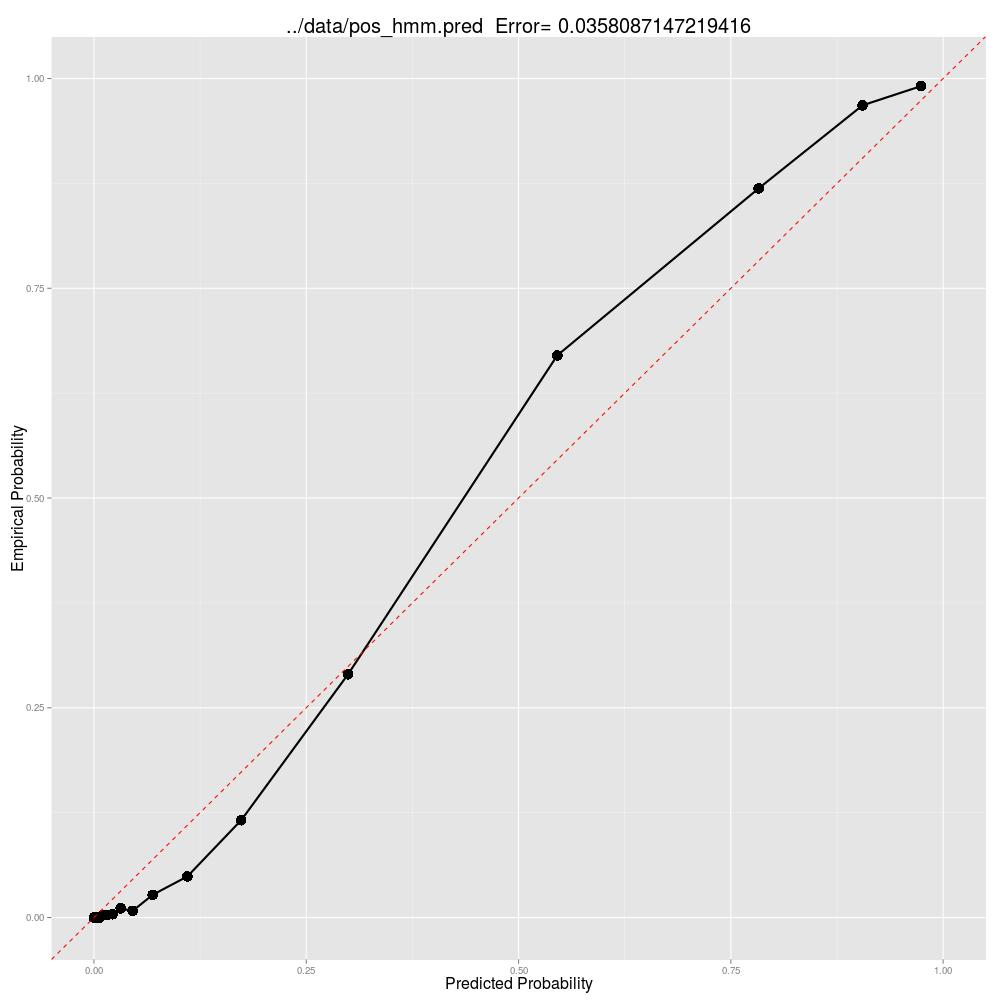
\includegraphics[width=\linewidth]{pos_hmm_pred.jpg}
  \caption{Calibration curve for HMM (POS), Acc = ??, CalibScore = ??}
  \label{fig:pos_hmm_pred}
\endminipage\hfill
\minipage{0.32\textwidth}
  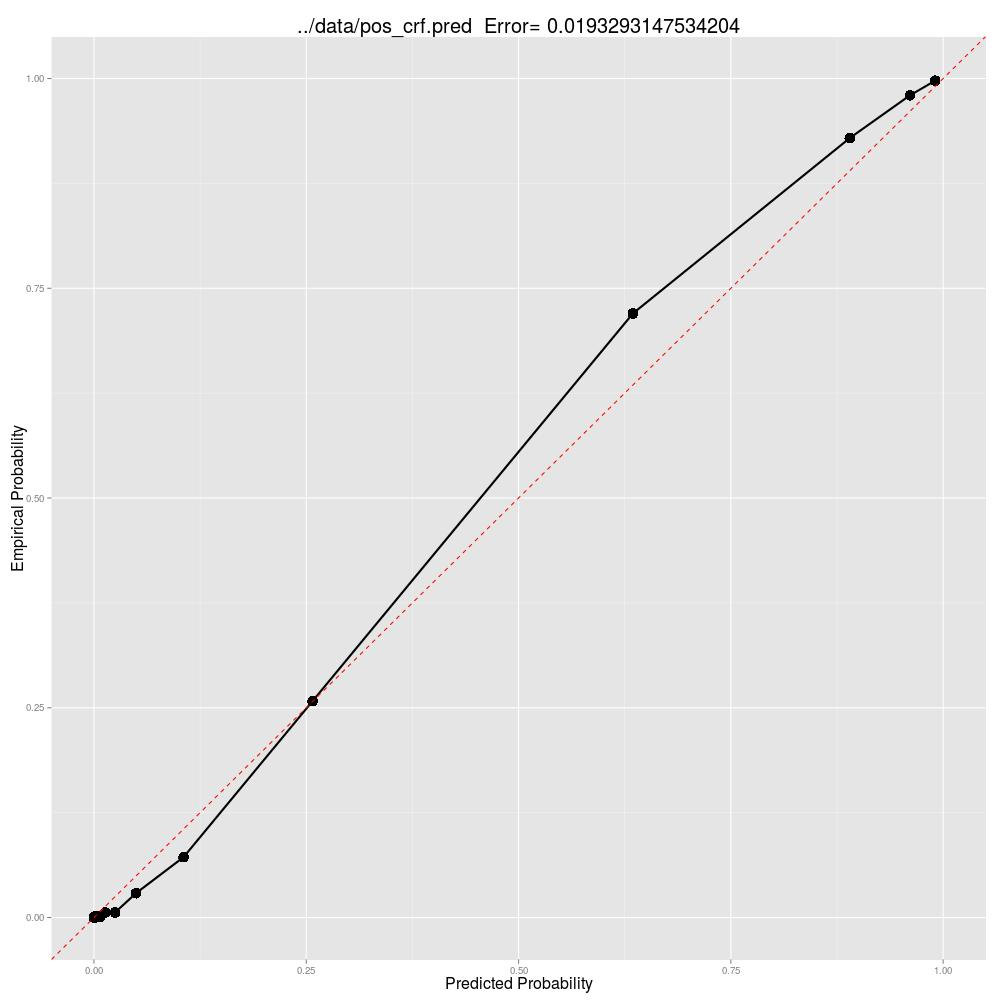
\includegraphics[width=\linewidth]{pos_crf_pred.jpg}
  \caption{Calibration curve for CRF-Basic (POS), Acc = ??, CalibScore = ??}
  \label{fig:pos_crf_pred}
\endminipage\hfill
\minipage{0.32\textwidth}
  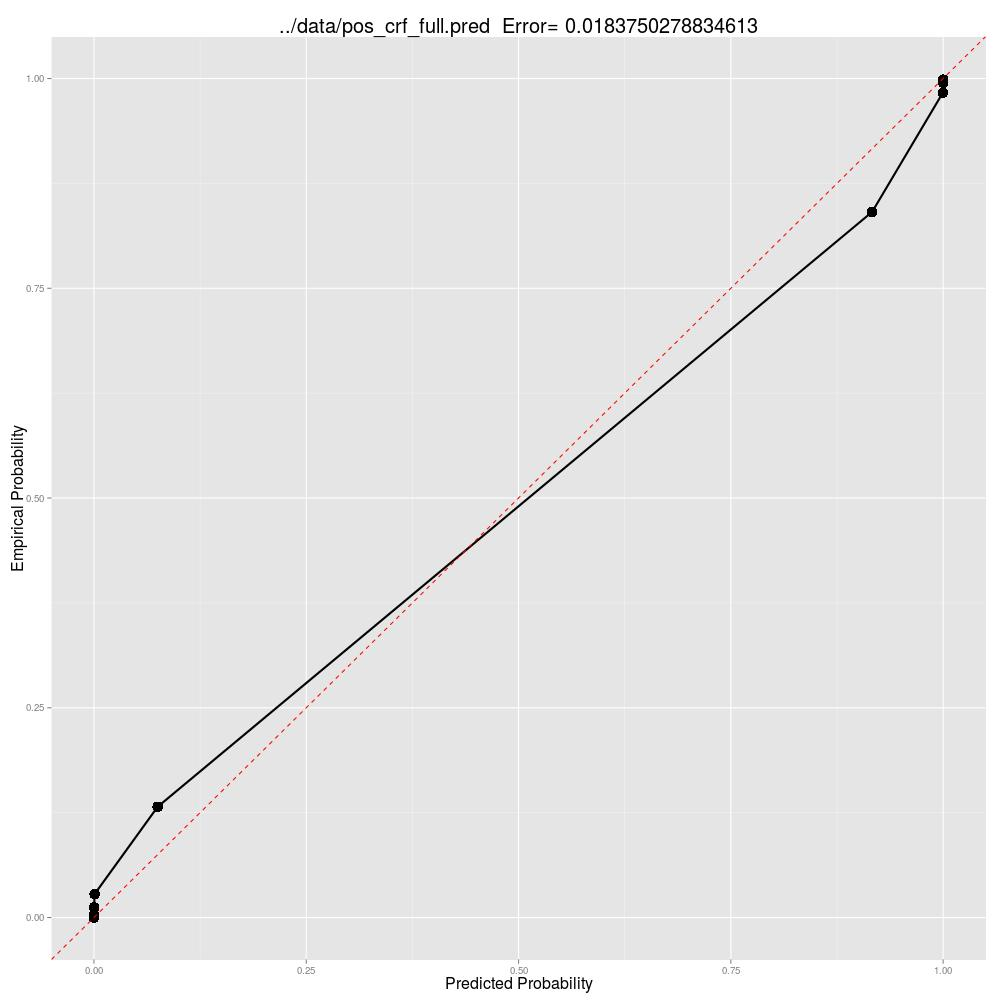
\includegraphics[width=\linewidth]{pos_crf_advanced_pred.jpg}
  \caption{Calibration curve for CRF-Advanced (POS), Acc = ??, CalibScore = ??}
  \label{fig:pos_crf_advanced_pred}  
\endminipage
\end{figure}

First of all, we compare a standard HMM with a CRF model with basic features (CRF-Basic). CRF-Basic contains only the emission features (pairs of the tag and the current token at each position) and the transition features (pairs of labels). Using CRF-Basic allows us to separate the characteristics of the model dependencies from the advantages of having features. The plots of calibration curves of the two models are shown in figure \ref{fig:pos_hmm_pred}. CRF-basic intuitively produces a better curve than HMM. Concretely, the miscalibration of CRF-Basic is roughly 1.8 times larger than that of HMM (0.019 vs. 0.035). Moreover, as seen from the distributions of points in the plots, CRF-Basic produces sharper predictions.

To measure fully the power of the CRF model, we add more features to it, including surrounding words, word shape, word length, prefixes and suffixes. This model, called CRF-Advanced, achieves a 96\% accuraccy on the task. It produces an extremely good posterior distribution. Figure \ref{fig:pos_crf_advanced_pred} shows its perfect calibration curve, which is just slightly off the perfect calibration line (calibration score = 0.018). 

\subsection{Twitter part-of-speech tagging}
\subsubsection{Data}

We repeat our comparision between HMMs and CRFs on a harder task, predicting POS tags for tweets. We use the ARK's Twitter POS data set (CITE NOAH), which consists of 1000 sentences for training, 327 sentences for development, 500 sentences for testing. The predictions we test is to predict whether a word has the ``V'' tag. 

\subsubsection{Data}

We conduct the same experiments as in Section BLAH BLAH and obtain similar patterns. CRF-Basic's miscalibration is about half HMM's (Figure \ref{fig:pos_tweet_hmm_pred}). On the other hand, equipped with better features, CRF-Advanced demonstrates a significant improvement from CRF-Basic, reducing further the miscalibration level by one half. It should also be noticed that CRF-Advanced does not give perfectly accurate predictions (87\% accuracy) but those are reliable predictions.   

\begin{figure}
\minipage{0.32\textwidth}
  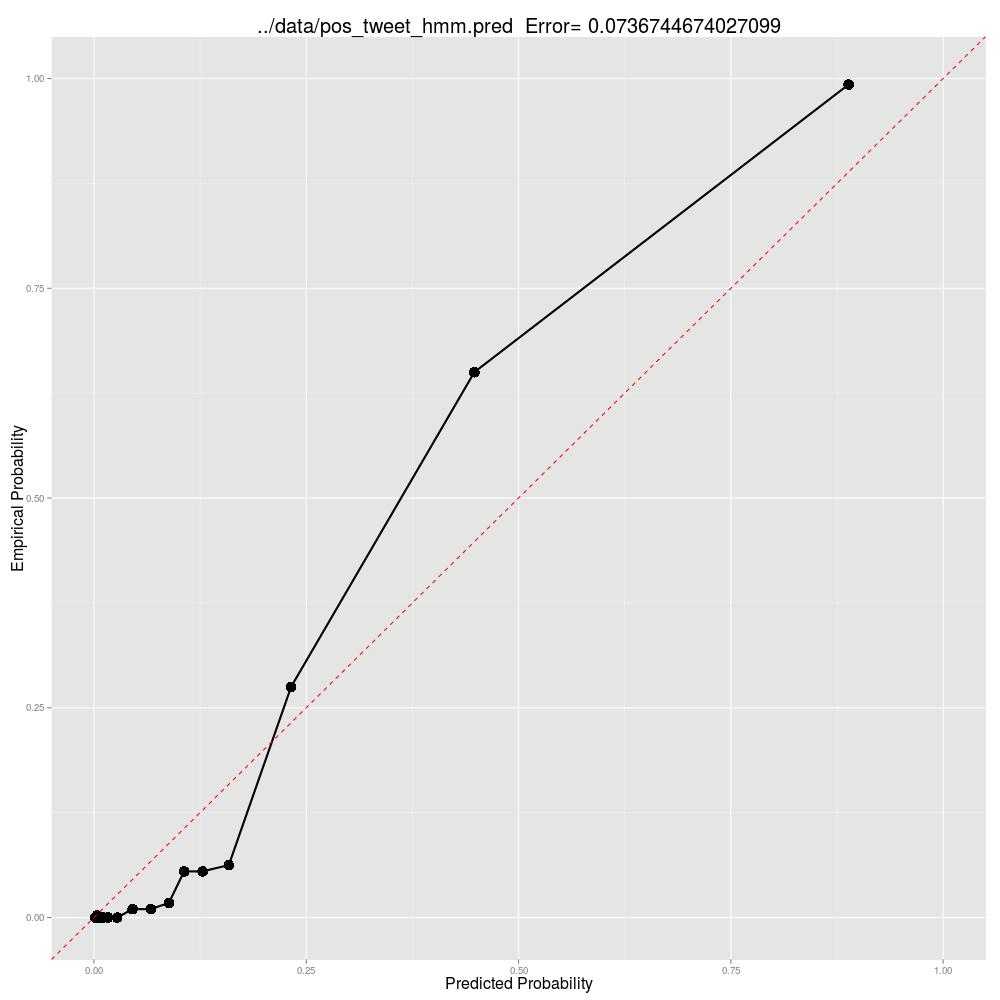
\includegraphics[width=\linewidth]{pos_tweet_hmm_pred.jpg}
  \caption{Calibration curve for HMM (POS Tweet), Acc = ??, CalibScore = ??}
  \label{fig:pos_tweet_hmm_pred}
\endminipage\hfill
\minipage{0.32\textwidth}
  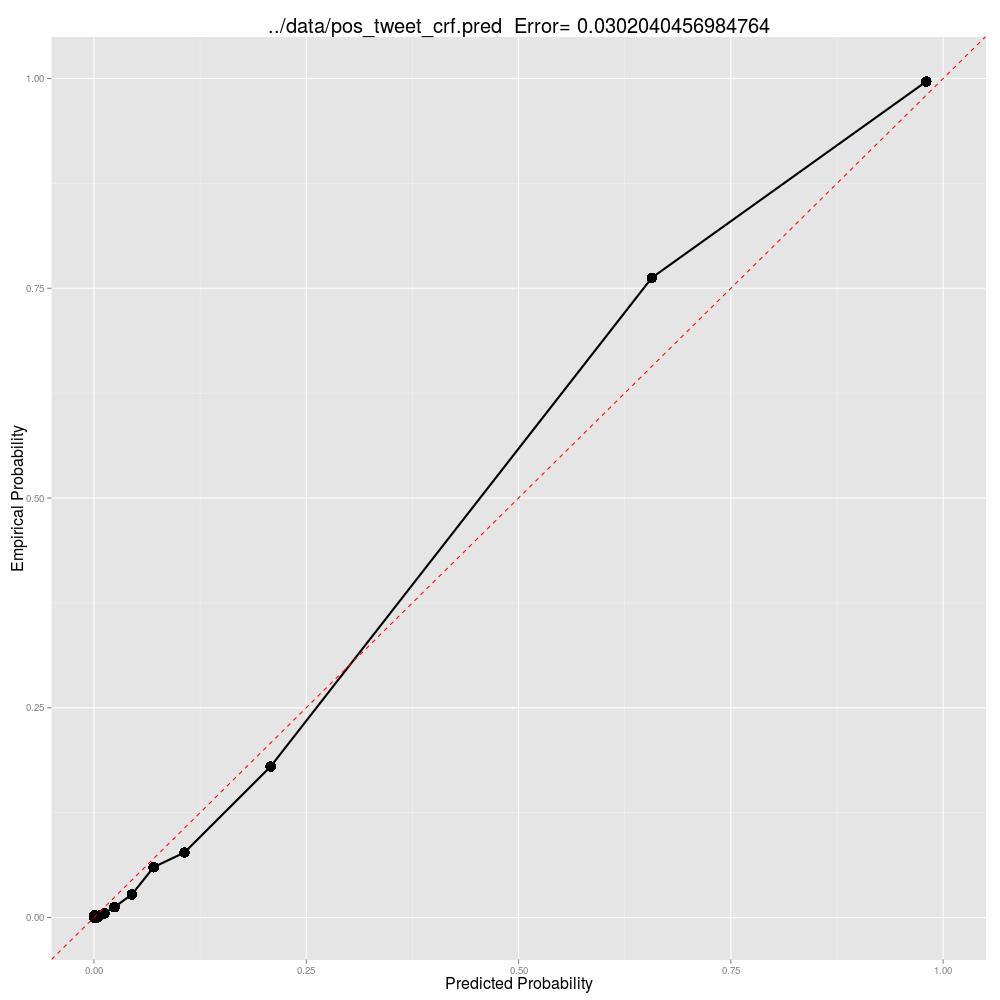
\includegraphics[width=\linewidth]{pos_tweet_crf_pred.jpg}
  \caption{Calibration curve for CRF-Basic (POS Tweet), Acc = ??, CalibScore = ??}
  \label{fig:pos_tweet_crf_pred} 
\endminipage\hfill
\minipage{0.32\textwidth}
  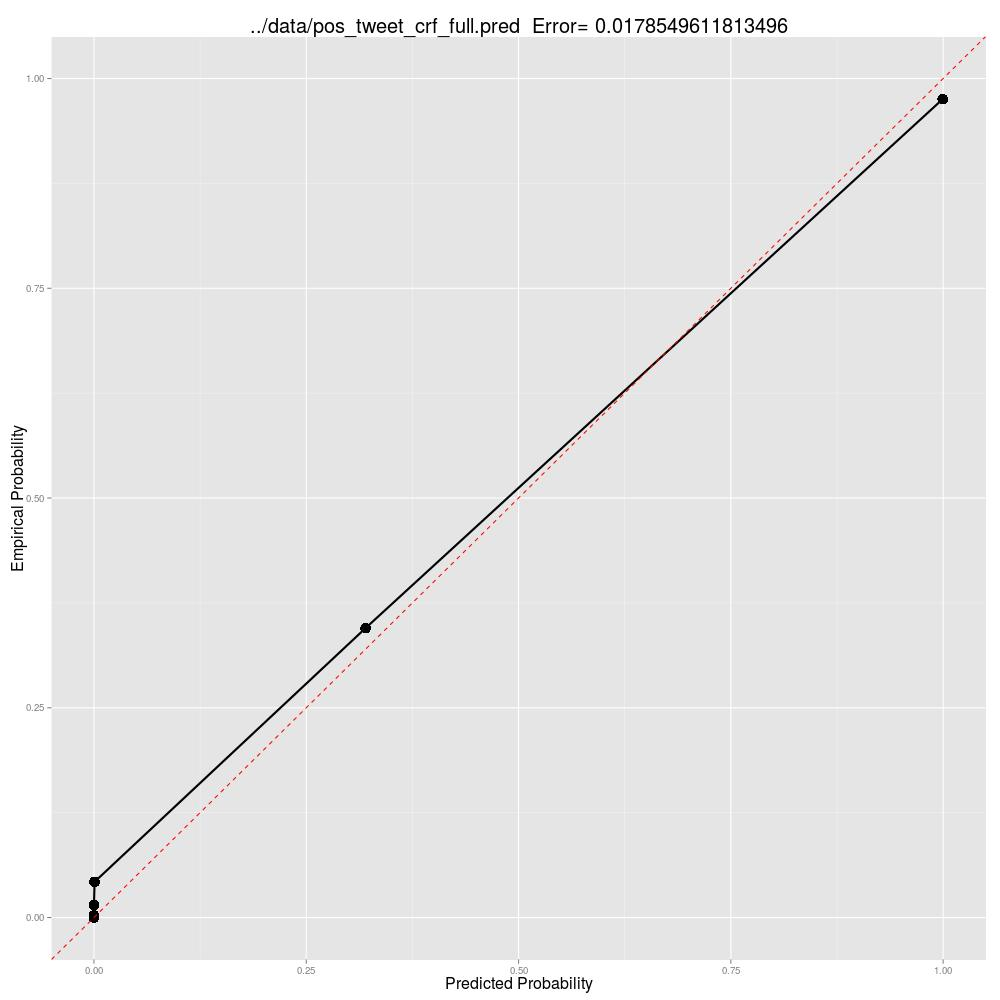
\includegraphics[width=\linewidth]{pos_tweet_crf_advanced_pred.jpg}
  \caption{Calibration curve for CRF-Advanced (POS Tweet), Acc = ??, CalibScore = ??}
  \label{fig:pos_tweet_advanced_crf_pred} 
\endminipage
\end{figure}


\section{Calibration analysis on synthesis data}

\subsection{Data}

Approximating calibration statistics is very difficult since the distribution of the true labels is unknown. Therefore, we investigate the behavior of calibration statistics on synthesized set of prediction-observation pairs that mimics common NLP data distributions. 

Each prediction-observation pair is generated as follows. First of all, the value of the prediction is drawn from a beta distribution. Then, the observation is obtained by sampling from a Bernoulli distribution whose parameter is a transformation of the value of the prediction. To obtain a perfectlycalibrated set of pairs, we use the identity transformation. For uncalibrated condition, we use this function $t(p)$:

\[
        t(p) =
\begin{cases}
  \max(0, p - k), & \text{if } 0 \leq x \leq 0.5 \\
  \min(0, p + k), & \text{otherwise}
\end{cases}
\]
where k $\in$ [0, 0.5].

\subsection{Effect of bin size on calibration score}

We investigate the the effect of varying the bin size on the value of the MSE calibration score. Theoretically, as we double the bin size, the score will not increase. This fact is obtain by using Jensen's inequality, leveraging the fact that the quaratic function is convex. In our experiment, we vary the bin size from $2^1$ to $2^16$ to calculate the MSE calibration score on a data set consists of $10^5$ pairs. Our result (Figure BLAH BLAH) supports the theoretical hypothesis. The score monotonically decreases as the bin size exponentally increases. We also alter the parameters of our beta distribution and witness the same pattern. We attempt to generalize this pattern to a contious range of bin size values. Figure BLAH BLAH portrays the behavior of the score of a perfectly calibrated predictor as the bin size goes from $10^3$ to $5.10^4$ with a step size of $10^3$. As we can see, although the points do not always monotonically decrease, we see a similiar trend as the log-scale plot. However, for an uncalibrated predictor, the score is much more unpredictable (Figure BLAH BLAH). 

\subsection{Effect of sample size on calibration score}

As pointed out by Foster (1998), we expect the calibration score of a perfectly calibrated predictor to go to zero as the sample size goes to infinity. We set up experiment to verify this fact. Using a range of sample size from $10^4$ to $5.10^4$, we compute the calibration score for three set of predictions: perfectly calibrated (PERFECT), uncalibrated using the function t(p) as true distribution with k = 0.1 (UNCALIB). For each experiement, we set the bin size to be the square root of the sample size. We observed distinguishing pattern between PERFECT and UNCALIB. The points in the CALIB's plot clearly approach zero while those of the UNCALIB's plot converge weakly. 




%%
%% Table of contents is mandatory, lists of tables and figures are 
%% mandatory if you have any tables or figures; must be in this order.
%%\listoftables                   % List of Tables
%%\listoffigures                  % List of Figures

%%
%% We don't handle List of Abbreviations
%% We don't handle Glossary

%%%%%%%%%%%%%%%%%%%%%%%%%%%%%%%%%%%%%%%%%%%%%%%%%%%%%%%%%%%%%%%%%%%%%%%%%
%% Time for the body of the dissertation
\mainmatter   %% <-- This line is mandatory

%%
%% If you want an introduction, which is not a numbered chapter, insert
%% the following two lines.  This is OPTIONAL:


%%
%% Some sample text
\chapter{A Introduction to Sheep}
Is there life afters:m:w sheep?~\cite{xyz}  Yes, I say there is.%\marginpar{Really?}

\section{Pulling the wool over your eyes}

Sheep are fabulou creatures.  The noises they make are truly stupendous
\cite{Bah}.  We also want to refer to figure \ref{fig:circle} here.
Here' some verbatim text to screw us up:

{\small
\begin{verbatim}
xxx := y;
xy := x;
\end{verbatim}
}

\begin{figure}
  \begin{center}
    \begin{picture}(300,200)
      \put(150,100){\circle{150}}
      \put(1,1){\framebox(298,198){}}
    \end{picture}
    \caption{A circle in a square.}\label{fig:circle}
  \end{center}
\end{figure}

\subsection{All about sheep noises}
Lots of text here just to fill up some space so we can be sure that we
really are double-spacing and doing all the other things that might be
necessary in formatting a dissertation to U.Mass. guidelines.  We're
also going to have another figure here, figure \ref{fig:disc}, just
for fun, and to make sure that the list of figures is formatted
correctly.  Now it's time for table \ref{table:somenumbers}.  We
really are going to need a third figure, figure \ref{fig:discs}, two
more tables, table \ref{table:morenumbers} and table
\ref{table:evenmorenumbers} and a fourth figure, figure
\ref{fig:circleanddisc}, just to really make sure.

\begin{figure}
  \begin{center}
    \begin{picture}(300,200)
      \put(150,100){\circle*{150}}
      \put(1,1){\framebox(298,198){}}
    \end{picture}
    \caption{A disc in a square.}\label{fig:disc}
  \end{center}
\end{figure}

\begin{table}[htbp]
  \begin{center}
    \caption{Some numbers.}
    \label{table:somenumbers}
    \begin{tabular}{|r|lll|}
      \hline
      & Minimum & Average & Maximum \\
      Type of Animal & Observed & Observed & Observed \\ \hline
      Cats & 12 & 20 & 24 \\
      Dogs & 20 & 20 & 20 \\ \hline
    \end{tabular}
  \end{center}
\end{table}

\begin{figure}
  \begin{center}
    \begin{picture}(400,200)
      \put(100,100){\circle*{150}}
      \put(300,100){\circle*{150}}
      \put(1,1){\framebox(398,198){}}
    \end{picture}
    \caption{Two discs in a rectangle.}\label{fig:discs}
  \end{center}
\end{figure}

\begin{table}[htbp]
  \begin{center}
    \caption{More numbers.}
    \label{table:morenumbers}
    \begin{tabular}{|r|lll|}
      \hline
      Type of Animal & Arms & Legs & Ears \\ \hline
      Person & 2 & 2 & 2 \\
      Dog & 0 & 4 & 2 \\ \hline
    \end{tabular}
  \end{center}
\end{table}

\begin{table}[htbp]
  \begin{center}
    \caption[Even more numbers; together with a caption long enough to ensure that multi-line caption formatting works correctly.]{Even more numbers; together with a caption long enough to ensure that multi-line caption formatting works correctly.  If you want a shorter caption to appear in the Table of Figures you're going to have to put the shorter caption in the \texttt{[]} as shown in this example.}
    \label{table:evenmorenumbers}

    \begin{tabular}{|r|lll|}
      \hline
      x & 1 & 1 & 1 \\ \hline
      y & 2 & 2 & 2 \\
      z & 3 & 3 & 3 \\ \hline
    \end{tabular}
  \end{center}
\end{table}

\begin{figure}
  \begin{center}
    \begin{picture}(400,200)
      \put(100,100){\circle{150}}
      \put(300,100){\circle*{150}}
      \put(1,1){\framebox(398,198){}}
    \end{picture}
    \caption{A circle and a disc in a square.  We want this caption to
      be very long to ensure that the formatting of very long captions
      is handled correctly.  The case of short captions has already
      been dealt with.}\label{fig:circleanddisc}
  \end{center}
\end{figure}



\subsubsection{Baahs}
\subsection{Even more about sheep noises}
\subsection{And yet more about sheep noises}

\section{What about wolves?}
What about wolves?\footnote{To be fair, some wolves are probably nice\ldots}

\section{What about shepherds?}
What about shepherds?  I don't really know, but I want some text here
to fill things in so that I can verify that everything is OK.%
\footnote{Some shepherds are good, some are bad. The reader is referred
  to Mary and The Boy Who Cried Wolf for further insight into this
  much-debated issue. (This needs to be a very long footnote so we can
  test the spacing between lines on a footnote.)}
\subsection{A subsection}
This is a subsection of the subsection about shepherds.
\subsection{Another subsection}
This is another subsection of that section.
\subsubsection{A subsubsection}
This is a subsubsection of that subsection that will in turn havae a
paragraph with a pair of subparagraphs.  I am aware that I shouldn't
have only one subsubsection in the subsection...
\paragraph{A Paragraph} 
This is the text associated with this paragraph.  I really want enough
text to make it look like a paragraph.  Baah, baah, baah.  Baah, baah,
baah.  Baah, baah, baah.  Baah, baah, baah.  Baah, baah, baah.  Baah,
baah, baah.  Baah, baah, baah.  Baah, baah, baah.  Baah, baah, baah. 
\subparagraph{A Subparagraph} 
This is the text associated with this subparagraph.  Baah, baah, baah.
Baah, baah, baah.  Baah, baah, baah.  Baah, baah, baah.  Baah, baah,
baah.  Baah, baah, baah.  Baah, baah, baah.  Baah, baah, baah. 
\subparagraph{Another Subparagraph}
Better not have subparagraphs without text in them.  Baah, baah, baah.
Baah, baah, baah.  Baah, baah, baah.  Baah, baah, baah.  Baah, baah,
baah.  Baah, baah, baah.  Baah, baah, baah. 
\paragraph{Another Paragraph}
Baah, baah, baah.  Baah, baah, baah.  Baah, baah, baah.  Baah, baah,
baah.  Baah, baah, baah.  Baah, baah, baah.  Baah, baah, baah.  Baah,
baah, baah.  Baah, baah, baah.  Baah, baah, baah.  Baah, baah, baah.
Baah, baah, baah.  Baah, baah, baah.  Baah, baah, baah.  Baah, baah,
baah.  Baah, baah, baah.  Baah, baah, baah.  Baah, baah, baah.  Baah,
baah, baah.  Baah, baah, baah.  Baah, baah, baah.

Baah, baah, baah.  Baah, baah, baah.  Baah, baah, baah.  Baah, baah,
baah.  Baah, baah, baah.  Baah, baah, baah.  Baah, baah, baah.  Baah,
baah, baah.  Baah, baah, baah.  Baah, baah, baah.  Baah, baah, baah.
Baah, baah, baah.  Baah, baah, baah.  Baah, baah, baah.  Baah, baah,
baah.  Baah, baah, baah.  Baah, baah, baah.  Baah, baah, baah.  Baah,
baah, baah.  Baah, baah, baah.  Baah, baah, baah.
\subsubsection{Another Subsubsection}
With some text.  Baah, baah, baah.  Baah, baah, baah.  Baah, baah,
baah.  Baah, baah, baah.  Baah, baah, baah.  Baah, baah, baah.  Baah,
baah, baah.  Baah, baah, baah.  Baah, baah, baah.  Baah, baah, baah. 

\chapter{Sheep and Grass}

\section{Introduction}

Grass is a wonderful food...  Baah, baah, baah.  Baah, baah, baah.
Baah, baah, baah.  Baah, baah, baah.  Baah, baah, baah.  Baah, baah,
baah.  Baah, baah, baah.  Baah, baah, baah.  Baah, baah, baah.  Baah,
baah, baah.  Baah, baah, baah.  Baah, baah, baah.  Baah, baah, baah.
Baah, baah, baah.  Baah, baah, baah.  Baah, baah, baah.  Baah, baah,
baah.  Baah, baah, baah.  Baah, baah, baah.  Baah, baah, baah.  Baah,
baah, baah.  Baah, baah, baah.  Baah, baah, baah.  Baah, baah, baah.
Baah, baah, baah.  Baah, baah, baah.  Baah, baah, baah. 

\chapter{A Wonderfully Long Chapter Title That Is This Long In Order
  to Test the Chapter Heading Stuff}
Note that we shouldn't really have a chapter heading with no body, so
here is a body for this chapter.  Baah, baah, baah.  Baah, baah, baah.
Baah, baah, baah.  Baah, baah, baah.  Baah, baah, baah.  Baah, baah,
baah.  Baah, baah, baah.  Baah, baah, baah.  Baah, baah, baah.  Baah,
baah, baah.  Baah, baah, baah.  Baah, baah, baah.  Baah, baah, baah.
Baah, baah, baah.  Baah, baah, baah.  Baah, baah, baah.  Baah, baah,
baah.  Baah, baah, baah.  Baah, baah, baah.  Baah, baah, baah.  Baah,
baah, baah.  Baah, baah, baah. 

\section{The antidisestablishmentarainism supercalifragilisticexpialidocious longlonglonglonglongword}

A \texttt{quotation}:

\begin{quotation}
Lorem ipsum dolor sit amet, consectetur adipiscing elit. Ut nibh orci, molestie
non vehicula ac, ultricies quis purus. Nunc euismod metus vel nulla sodales quis
tempus nisi varius. Sed ornare pulvinar bibendum. Ut egestas mollis nisi vel
cursus.
\end{quotation}

\dots and a \texttt{quote}:

\begin{quote}
Ut dolor libero, blandit tristique accumsan non, viverra a magna. Sed pretium
sollicitudin neque, sit amet ornare lorem convallis ac. Fusce mollis gravida
aliquam. Nullam vulputate turpis vitae orci porttitor auctor. Donec in auctor
erat.
\end{quote}



%% End of body
%%%%%%%%%%%%%%%%%%%%%%%%%%%%%%%%%%%%%%%%%%%%%%%%%%%%%%%%%%%%%%%%%%%%%%%%%%%%%%%

\appendix
\chapter{THE FIRST APPENDIX TITLE}
...
\chapter{THE SECOND APPENDIX TITLE}
...

%%
%% Beginning of back matter
\backmatter  %% <--- mandatory

%%
%% We don't support endnotes

%%
%% A bibliography is required.
\interlinepenalty=10000  % prevent split bibliography entries
\bibliographystyle{thesis}
\bibliography{thesis}
\end{document}

%%% Local Variables: 
%%% mode: latex
%%% TeX-master: t
%%% End: 
